\chapter{Protocol Runtime}
\label{sec:protocol_runtime}
In this section we explore the Rust implementation of Reo-generated protocol objects. Rather that generating the needed structures and behaviour from scratch each time, the Rust back-end follows the precedent of the well-established Java back-end and relies on a single, re-usable dependency for the work common to all protocols. Here, we explore the implementation of this \textbf{Reo-rs} library, picking up where we left off from the generation step in Chapter~\ref{sec:imperative_form} above.

\section{Examining the Java Implementation}
\label{sec:java_examined}
The work of this project can draw from the efforts of previous work on the Reo Compiler. The Java implementation in particular has seen the most frequent and recent updates. This section treats the Java code generator as a touchstone for Reo-generated application code in general. We give a brief overview of the properties inherent to the generated code, and consider the effects of projecting the underlying ideas to the Rust language.

\subsection{Architecture}
Fundamentally, the generated code adheres closely to Reo's literature, revolving around the interplay between \code{Port} and \code{Component} objects. From the perspective of a developer looking to integrate a generated Java protocol into their application, the entry point is the \code{Protocol} component (where `Protocol' is the name of the associated Reo connector).

Running a system requires an initialization procedure: (1) a \code{Port} is instantiated per logical port, (2) a \code{Component} is instantiated per logical component, and (3) pairs of components are linked by overwriting a port-field for both objects with the same instance of \code{Port}. To get things going, each component must be provided a thread to enter it's main loop; in idiomatic Java, this manifests as calling \code{new Thread(C).start()} for each component \code{C}. A simplified example of the initialization procedure is shown in Listing~\ref{listing:java_gen_1} for the simple `sync' protocol which acts as a one-way channel. In this example, the ports are of type \code{String}.


\begin{listing}[ht]
	\centering
	\inputminted[]{java}{java_gen_1.java}
	\caption[Reo-generated Java protocol initialization.]{A simplified example of initialization for a system centered around a \code{Sync} protocol object, which acts as a channel for transmitting objects of type \code{String}. Both ports and components are constructed before they are `linked' in both directions: each port stores a reference to its components, and each component stores references to its ports. The system begins to \textit{run} when each component is given a thread and started.}
	\label{listing:java_gen_1}
\end{listing}


In a sense, this implementation primarily hinges on \code{Port} as a communication primitive between threads, and equivalently, between components. For matters of concurrency, operations on port-data involves entering a \textit{critical region}. In contrast, \code{Components} are used only to store their ports and to be used as name spaces for their \code{run} function which implements their behavior (which corresponds to RBA rules in the case of the protocol component). Essentially, anything that interacts with \code{Port} objects can reify a logical component, whether or not this is done by an object implementing the \code{Component} interface.

\subsection{Behavior}
The representation of protocol rules is very intuitive; a rule is implemented as a block of code which operates on a component's ports. Once generated into Java, the only obvious sign that a component was generated from Reo is its linkage to multiple other components\footnote{The distinction between `protocol' and `compute' components is tenuous at the best of times. If compute components are allowed to interact directly with one another, the distinction observed here disappears also.}. The (simplified) generated \code{Component} code of the `sync' protocol from the previous section is shown in Listing~\ref{listing:java_gen_2}. This demonstrates that rules are indeed \textit{commandified}, in that their behavior is encoded in discernible structures (appropriately called \code{Command}).

The behavior and structure of a component go together, and are generated by Reo at a relatively granular level. As such, the encoding of memory cells is natural also. Memory cells can be found next to ports in the fields of a \code{Component}.

\begin{listing}[h!]
	\centering
	\inputminted{java}{java_gen_2.java}
	\caption[Reo-generated Java protocol class of the sync connector.]{A simplified example of a Reo-generated Java protocol class for the \textit{sync} connector. By convention, it is started by invoking \code{start}, which is a method inherited from the \code{Runnable} interface which \code{Component} extends. This method assumes that all ports are correctly initialized and linked to another `compute' port. Its RBA-like behavior comes from an array of guards and commands which it iterates over in a loop, firing rules as possible forever.}
	\label{listing:java_gen_2}
\end{listing}

\subsection{Observations}
\label{sec:java_observations}
It is very easy to see the correspondence between a generated Java protocol and its Reo definition. This carries over to how components and ports are used by an application developer. Next, we consider their higher-level properties that follow from the observations in the previous sections:




\begin{enumerate}
	\item \textbf{Protocol Event Loop}\\
	Protocols are fundamentally \textit{passive} in that they do not act until acted upon. Nevertheless, protocols each have their own dedicated thread that waits in a loop for a \textit{notification} from its monitor. Notifications originate from a component's own \code{Ports} in the event of a \code{put} or \code{get} invocation. For this reason, protocols and components are related in both directions, afforded by setting a port variable in one direction, and functions \code{setProducer} and \code{setConsumer} in the other.
	
	True to the intuition behind the RBA model, the protocol must \textit{check} which (if any) commands can be fired, and keep spinning, trying rules while \textit{any} guard is satisfied. This is unfortunate, as this approach requires guards to be evaluated repeatedly. As the protocol relies on the actions of other components to make progress, it is counter-productive for it to spend a lot of system resources evaluating guards to \textit{false}. In cases where threads must share processor time, the excessive work of the protocol component will begin to get in the way of other components making progress, in turn leading yet more guards to evaluate to \textit{false}.
	
	\item \textbf{Reference Passing}\\
	Java is a managed programming language whose garbage collector is central to how the language works. To support the transmission of arbitrary data types, \code{Port} is generic over a type. The language only supports this kind of polymorphism for objects. Unlike primitives (such as \code{int}), the data for objects is stored on the heap and is garbage collected by the Java Virtual Machine. Variables of such objects are therefore moved around the stack by \textit{reference}. Moving and replicating values is cheap and easy, as they always have a small (pointer-sized) representation on the stack.
	
	A minor drawback is the need for indirection when performing operations that need to \textit{follow} the reference. For example, comparing two \code{Integer} objects requires that the \code{int} primitives backing them on the heap be retrieved and compared. Equality is an example of an operation that the Reo protocol thread can be expected to perform frequently. The cost of this indirection depends on a myriad of factors, but is at its worst when it results in new, spread-out locations each time. This case might arise, for example, if the \code{Sender} continuously created new \code{Integer} objects and sent them through its port. Another drawback is the \textit{requirement} to allocate primitives on the heap before they can be sent through a port. This is not usually a problem in the case of Java, as in practice, almost everything is going to be stored on the heap with or without Reo.
	
	This aspect of the generated Java code will require the most change for the Rust version, as Rust has a very different model for memory management; it does not use a garbage collector by default, and structures are stored first and foremost on the \textit{stack} as in the C language.
	
	\item \textbf{Two Hops for Data}\\
	As protocols are components like any other, even the most trivial of data-movements require values to hop at least twice: into the protocol, and out of the protocol. Fortunately, as stated above, the cost of the `hop' itself is trivial, as it will always be a small reference. The problem is the time delay \textit{between} the hops, as it will often involve actions of three distinct threads in series (with the protocol in the middle). 
	
	\item \textbf{Vulnerable to User Error}\\
	The construction and linking of components with ports is not something the protocol itself is concerned with. Indeed, \textit{every} component assumes that their port-variables will be initialized by their environment. At the outermost level, this environment is in the application developer's hands. Components make no attempt to verify that they are correctly linked according to the specification; currently, there is not any infrastructure in place to support this checking if it were desired. As a result, it is possible make mistakes such as fusing two of a protocol's ports into one. Whether this is a problem worth solving depends on the burden of responsibility that Reo intends to place on the end user. These difficulties cannot be completely avoided, but approaches exist to minimize these opportunities for mistakes.
	
	While ports are clearly directional `from the inside out' (ports store distinct references to their producer and consumer components), the same is not so `from the outside in'. Neither of a port's components is prevented from indiscriminately calling \code{put} or \code{get}. The assignment of a port's values for `producer' and `consumer' component is in user-space also. As a consequence, these fields may not agree with the components that interact with the ports at all. In fact, any number of components may store a reference to a port, each arbitrarily calling \code{put} and \code{get}. If done unintentionally, this would lead to \textit{lost wakeups}; the thread blocking for a notification after calling acting on the port is not the same as the thread receiving the notification. Solutions can be conceived to \textit{wrap} ports in objects that constrain the API of a port to one of the two `directions'. However, without affine types, there is no obvious way to ensure the \textit{number} of components accessing a port is correct. In Rust, limiting these accesses becomes feasible.
	
	\item \textbf{Port Data Aliasing}\\
	In Reo, it is common for connectors to replicate port data. Owing to the nature of Java, this is currently achieved by duplicating references, where replication is also known as \textit{aliasing}. For immutable objects, aliasing has no observable side effects, and thus does not threaten Reo's value-passing semantics. However, Reo ports permit instantiation with \textit{any} object-type. Even if the operations are thread-safe, this causes \textit{incorrect} behavior, as a component might observe their data changing seemingly under their feet. Worse still, objects which are not thread-safe can cause undefined behavior. This is a result of Java's view on memory safety having inverted priorities to Rust. In Java, operations are unsafe by default, and the programmer must go out of their way to protect themselves from data races, access of invalid memory and corruption. In Rust, the \textit{ownership system} is based on the prohibition of mutably-aliased variables. Achieving replication in Rust will require some effort to convince the compiler of safety before a program will compile.
	
	\item \textbf{Non-Terminating Protocols}\\
	Currently, Reo-generated protocol objects loop forever unless they raise an exception and crash. For protocols that can perform actions with observable side-effects in the absence of other components, this is perhaps a good idea. However, in the majority of realistic cases, protocols are indeed passive, and cannot do meaningful work as the only component. Reo semantics tend to reason about \textit{infinite} behaviors. However, real programs often do \textit{end}, and it is desirable that the program's exit is not held up by an endlessly-blocked protocol thread.
	
	\item \textbf{Protocol Components Cannot be Composed at Runtime}\\
	(TODO is this the place to explain this?)
	Ports allow data to move from the putter (or `producer') and getter (or `consumer') components as an \textit{atomic} operation by delaying \code{put} or \code{get} operations until their counterpart is called also. This causes problems for the implementation of RBAs with rules whose guards are predicated by the data they move. How can a protocol \textit{decide} if it should fire as a function of values it can only obtain \textit{by} firing? This ability to reason about the future is currently still a luxury limited to models such as TDS. The Java implementation gets around this problem by introducing \textit{asymmetry} between `compute' and `protocol' components. Protocols are allowed to \textit{cheat}. The \code{Port} object has additional operations to inspect a value without consuming it: \code{peek} and \code{hasGet}. However, this asymmetry means that composing two Java protocol components (by linking them with ports) does \textit{not} result in a component with their composed behavior. Solving this problem in earnest requires continuously-connected protocols to reason about their distributed state, which is a problem beyond the scope of this work. Reo's relationship with \textit{liveness properties} is explored in Section~\ref{sec:api}.
	
	\item \textbf{Sequential Coordination}\\
	The Java implementation is structured such with \textit{ports} being the critical region between components. As protocols have multiple ports, at first glance it may appear that coordination events could occur in parallel. However, no communication through protocol $P$ happens without the single thread in $P$'s \code{run} method. Indeed, \code{put} and \code{get} operations can be \textit{started} in parallel by the boundary components, but $P$ can only complete it's half of these operations sequentially.
	
\end{enumerate}

\section{Requirements}
The Reo compiler's Java code generator were examined in Section~\ref{sec:java_examined}, resulting in the extraction of some high-level observations, enumerated in Section~\ref{sec:java_observations}. In this section, we lay out the requirements for Reo-rs. These requirements serve a dual purpose; firstly, it serves to structure the argumentation in sections to follow, primarily linking design choices together by providing over-arching motivations. Secondly, it provides a lens through which to view the work to follow, particularly for helping future readers to identify differences in their requirements such that different decisions can be made.

\subsection{Requirements Defined}
First, we enumerate and name the most vital \textbf{functional requirements} for the Reo-rs library. These requirements determine \textit{what} functionality must be available to the end user of protocols and ports, and which safety properties must be preserved.

\begin{enumerate}
	\item[$\boldsymbol{R^F_{correct}}$] Preserve Reo's value passing semantics. No user interaction should contradict these semantics. This precludes data races as a result of \textit{mutably aliasing} resources which the user considers to be independent values.
	
	\item[$\boldsymbol{R^F_{init}}$] Prevent the protocol from being initialized in an inconsistent state. Prevent port objects from being unitialized, unsafely accessed in parallel, or incorrectly connected to the protocol.
	
	\item[$\boldsymbol{R^F_{ffi}}$] Facilitate a foreign function interface with other systems languages C and C++. Ports and protocol objects should be accessible from those languages as well as Rust, such that they can be constructed, used and destroyed.
\end{enumerate}

Next, we enumerate the requirements which are \textit{qualitative}. By their nature, they cannot be met absolutely. Rather, they serve to guide the design of the implementation to prioritize the design decisions they affect. For those associated with run time, Chapter~\ref{sec:benchmarking} will assess the extent to which these goals are met.

\begin{enumerate}
	\item[$\boldsymbol{R^N_{data}}$] Allow the transmission of large data types without requiring the user to move the from the stack to the heap. Minimize the number of times data must be \textit{moved} in memory such that data transmission remains performant for types with large representations.	
	
	\item[$\boldsymbol{R^N_{fast}}$] Minimize the overhead of \textit{control
	operations} for the protocol object to route payloads and perform bookkeeping. In particular, minimize the cost of \textit{evaluating} the rules before one is selected for firing.
	
	
	\item[$\boldsymbol{R^N_{end}}$] Facilitate the protocol object being destroyed and its resources freed. Facilitate a means of detecting termination which is correct and ergonomic.
\end{enumerate}

\subsection{Requirements Evaluated}
\hl{TODO}


\begin{enumerate}
	\item[$\boldsymbol{R^F_{correct}}$] Values passing through ports preserve value passing. This is achieved even in the presence of reference-passing optimizations `under the table' by leaning on the same philosophy that Rust uses to prevent data races: prohibit mutable aliasing. Objects are only aliased (accessible via multiple bindings) if they should be identical. Section~\ref{sec:port_operations} explains how we prohibit aliasing into and out of the protocol by relying on value-passing port operations. On the other hand, Reo-rs aliases values, but only \textit{until} they are mutated. Section~\ref{sec:memory_cells} explains how memory values are safely aliased. \hl{TODO refer to the section that treats transform functions}
	
	\item[$\boldsymbol{R^F_{init}}$] Section~\ref{sec:user_facing} explains how users are shielded from the granular initialization procedure by exposing an API with explicit constructor functions \code{build} and \code{claim} of protocols and ports respectively. Protocol objects are extensively customizable by the expressiveness of \textit{imperative form}, with which \code{build} is parameterized. At the same time, these structures are kept internally-consistent by the preservation of invariants, and relying on \code{build} as the only user-facing means of instantiation.
	
	\item[$\boldsymbol{R^F_{ffi}}$] C and C++ foreign-function interfaces are provided by relying simply declarations with the C ABI where possible. As C cannot support Rust's notion of generics, where necessary, the \code{ffi} module provides generic-free alternatives for data types and functions where generics are represented as data instead. Reo-rs can thus be compiled once into either a statically- or dynamically-linked library for use in these other languages without any additional runtime overhead.
	
	\item[$\boldsymbol{R^N_{data}}$] Reo-rs facilitates the transmission of any fixed-size data-types by value. This permits but does require data to be heap-allocated. Sections~\ref{sec:data_exchange} and~\ref{sec:memory_cells} explains how Reo-rs has a value-passing API, but relies on reference-passing to minimize the number of times values are moved in memory.
	
	\item[$\boldsymbol{R^N_{fast}}$] Section~\ref{sec:chosen_design} explains Reo-rs coordinates the actions of multiple threads while minimizing the overhead of inter-thread communications. Section~\ref{sec:minimizing_the_bottleneck} explains how meta-operations are represented such that they can be batched, allowing the coordinator to reduce the overhead of processing rules for firing.
	
	
	\item[$\boldsymbol{R^N_{end}}$] Section~\ref{sec:chosen_design} explains how protocol objects are not given their own threads, trivially facilitating termination detection if no ports remain to interact with it. Section~\ref{sec:construction_and_destruction} describes how protocol structures are implicitly cleaned up once all of their ports are destroyed. 
\end{enumerate}

\section{Protocol Runtime}
\label{sec:protocol_runtime}
Here, we explore the Reo-rs library implementation which provides user-facing types that work together to behave as coordination primitives at runtime in accordance to the imperative-form-like \code{ProtoDef} used to configure them.

First, Section~\ref{sec:user_facing} explains the functionality of Reo-rs through the lens of the user-facing API. Beyond this surface level, there is a large design space for implementing the internals. As such, this project necessitated the exploration of several of these possibilities before settling on a design. Section~\ref{sec:chosen_design} begins by summarizing these possibilities and motivating the choice for this work. Section~\ref{sec:protocol_object_architecture} details how this design is laid out as more concrete type definitions in the library (most of which the user will never see). Finally, Section~\ref{sec:behavior_implementation} describes how these structures interact to emerge as coordination.

\subsection{Application User Interface}
\label{sec:user_facing}
The Reo compiler generates protocol descriptions in imperative form, which then are transformed by Reo-rs into runnable objects. The user therefore interacts mostly with Reo-rs itself, and Reo provides only the entry point for building particularly instances of protocol object. In this section we explain which functionality of Reo-rs is user-facing, focusing primarily on which requirements are satisfied.


\subsubsection{Construction and Destruction}
\label{sec:construction_and_destruction}
Reo-rs is built to interface with the Reo compiler, but it is not dependent on it. The entry point for protocol objects is the \code{ProtoDef} type, which is a concrete realization of the (logical) imperative form. Instances of this type are visible in Listings~\ref{listing:reo_out} and~\ref{listing:reo_out2}, but its definition is omitted for brevity (available in the source code). Regardless of whether the constructed \code{ProtoDef} was Reo-generated, it is instantiated along with any initial memory cells (in the \code{MemInitial} structure) to produce a \code{ProtoHandle}. This type has a small, pointer-sized shallow representation (ie. 32 or 64 bits) to the \code{Proto} structure on the heap. The handle is opaque to the user, at first glance offering no functionality other than to replicate the handle (aliasing the \code{Proto}) or to destroy the handle (in Rust this is done implicitly by letting its binding go out of scope, or explicitly by invoking~\code{mem::drop}). Once the last handle to a \code{Proto} instance goes out of scope, its resources are freed. This is achieved by relying on the Rust-idiomatic \code{Arc} type, (`atomic reference-counted') for the definition of \code{ProtoHandle}.

The system cannot come to life until the user acquires some of the protocol's \textit{ports}. In Reo-rs, there is indeed a singular type for a port object (\code{PortCommon}), but the user does not acquire it directly; instead, users are able to create and destroy two distinct types that \textit{wrap} \code{PortCommon}: \code{Putter} and \code{Getter}. In this manner, the \textit{direction} of the logical type is enforced; only \code{Putter} can put, and only \code{Getter} can get. Both are created by the \code{claim} function, which is invoked parameterized with (1) a \code{Protohandle}, (2) the data type of the port as a \code{TypeInfo}, and the name of the port to identify it (`name' is a string, corresponding to the one used in the definition of the \code{ProtoDef}, exemplified in Listing~\ref{listing:reo_out}). In this manner, the \code{Proto} is involved in the creation of these port objects and is able to enforce that (1) ports have the correct \textit{direction}, (2) no logical port may have more than one putters or getters at a time, and (3) the port type is instantiated with the correct \textit{data type}. All of these types and operations are also perfectly thread-safe, relying on the proto-lock, to be discussed in Section~\ref{sec:protocol_object_architecture}. When used from Rust, \code{Getter} and \code{Putter} have generic type paramters that do not influence their memory representation, but rather enforce that the data-type with which they are claimed matches that used in puts and gets. These generic arguments are not available in C; instead, a variant of these port types are available that store the \code{TypeId} as data, and reflect on it whenever putting or getting to preserve safety.

Putters and getters store replicas of their proto-handles (by necessity), which can be examined for subsequent claims; this means that the original \code{ProtoHandle} can be safely discarded. The \code{Proto} is destroyed only when all proto-handles \textit{and} all of its ports are destroyed. \code{Proto} is also involved in the destruction of ports, which affords the user discarding and \textit{reclaiming} ports at will. These port objects can also be treated as data, sent across threads, stored in buffers or moved to the heap. However, there is no safe means of \textit{replicating} a port object, ensuring that no two threads can be putting or getting on the same logical port at once.


\subsubsection{Port Operations}
\label{sec:port_operations}
Putters and getters rely on Rust's \textit{mutability} rules for ensuring that at most one thread is accessing each of a protocol's logical ports at a time; concretely, \code{Get} has method \code{get} with signature \code{fn~get(\&mut~self)~->~T}, and likewise for \code{put}. Otherwise, the operations of these two types are distinct.

Getters offer \code{get}, which blocks the calling thread, and returns an object of type \code{T}, where \code{T} is the data type with which the putter was claimed. Other variants of this method exist which may be more ergonomic for the user depending on the circumstance. \code{get\_timeout} takes an extra \code{Duration} parameter, and will attempt to return once the duration has elapsed without the port being involved in a rule firing. Rather than \code{T}, this method returns \code{Option<T>}, where the \code{Option::None} variant communicates that timeout was exceeded before a value was acquired. For cases where the getter wishes to participate in a rule firing, but for whatever reason does not actually want the data, \code{get\_signal} is available; this method behaves like \code{get}, but returns no value. Finally, \code{get\_signal\_timeout} behaves as expected, returning a boolean \code{true} to communicate whether the getter participated in a rule firing before timing out; in either case, no element of the port's data type is returned.

Putters also have variants of \code{code} available that mirror those of the getter; \code{put\_timeout} behaves as expected. However, putters do not have a parallel to the getters' \code{get\_signal}. At the moment the datum is offered, it is unknown whether any getters (directly involved in the firing, or indirectly acquiring it after it is stored in the protocol's memory) will want the data. As putters `go first', they are subservient to the choice of the getters, and must be ready to deal with the situation in which their put-datum was involved in a rule firing, but not consumed. Reo-rs attempts to avoid the costs of creating or destroying port-data values wherever possible, as these operations may be arbitrarily expensive. As such, rather than the expected signature of \code{fn(\&mut self, T)}, the \code{put} method returns a value of type \code{Option<T>}; if their value is not consumed, it is instead \textit{returned} to the putter. The expectation is that this option is beneficial to the user, they are able to re-send the same datum, or use it elsewhere; Here, a return value of \code{Option::None} communicates that the value was consumed. If the putter is not concerned with retaining an unconsumed value, the method variant \code{put\_drop} is available which returns the datum regardless of the actions of getters.


Both putters and getters transfer their data into and out of the stack frames of their port operations respectively \textit{by value}. Owing to its focus on resource affinity, Rust relies on its \textit{move semantics} for both (a) relocating bytes in memory, and (b) transferring a semantic resource binding. For cases where the relocation of bytes is not necessary, LLVM can often be relied upon to optimize the memory movements away, passing consumed resources by reference `under the hood'. However, these optimizations are not guaranteed. Users of the Rust language have grappled with this shortcoming for years, but the search for a satisfying solution remains an open problem~\cite{matsakis_2015}. For us, this problem it presents itself when defining our API. Neither of the available options satisfy all of our requirements; $\boldsymbol{R^F_{correct}}$ asserts that we cannot rely on reference passing from user-controlled code, as it becomes impossible to enforce Reo's value passing semantics. On the other hand, relying on Rust's move semantics has the potential to insert up to two copies of our values, working against our satisfaction of $\boldsymbol{R^N_{data}}$. Our choices are as follows:

\begin{enumerate}
	\item \textbf{Value passing.}\\
	We expose safe functions \code{put} and \code{get} to consume and return data \textit{by value}, guaranteeing correctness. Depending on the compilation environment, it may require up to two moves of the data.
	
	\item \textbf{Reference passing. User provides correctness.}\\
	We expose unsafe functions \code{put\_in\_place} and \code{get\_in\_place} to consume and return data \textit{by reference}, relying on the user's care to initialize or drop the corresponding value themselves. According to Rust's idiom, these functions are marked with the \textit{unsafe} keyword, moving the burden of preserving correctness to the user. Their use necessitates explicitly wrapping them in \code{unsafe} blocks, such that it is easy to identify weak spots in a program's correctness.
	
	These functions are ideal for a \textit{foreign function interface} (to C, for example), for which \textit{unsafe} is often necessary anyway.
	
	\item \textbf{Value pass a `referring' type.}\\
	The user passes type \code{Q} through ports by value, where \code{Q} \textit{represents} the real type, \code{T}, ie. the user re-interprets what Reo-rs will consider to be the port's data type. As far as the protocol is concerned, \code{put} and \code{get} is called as in case (1).
	The simplest approach is to mimic that of Java, passing type \code{Box<T>}, representing an owned heap-allocated resource as an \textit{owned pointer}. Other approaches may be simple (eg: transmitting an integer which keys into a shared map) or arbitrarily complicated (Several Rust libraries exist for decoupling an object's data from its \textit{ownership}, such as \code{rent\_to\_own}, \code{managed} and \code{swapper}\footnote{These libraries are publically available on \url{crates.io}.}). 
\end{enumerate}

Options (1) and (3) are already supported by the methods described thus-far. To cover the remaining case, we rely on Rust's \textit{unsafe} API idiom to expose this trade-off for users to make on a case-by-case basis. Additional `raw' method variants are available which mimic Rust's move semantic by consuming and producing port data at the source and destination of a provided \textit{pointer}. Users are responsible for safely initializing and uninitializing the datum appropriately to avoid leaking memory or encountering undefined behavior. As is the idiom, these functions are explicitly marked with \textit{unsafe}, communicating to users that their use requires additional care to use these functions in accordance with their documentation. This option is therefore well-suited to the foreign-function interface with C.

In sections to follow, we ignore this complication and presume the safer value-passing variants are used only.

\subsubsection{Interface with C and C++}
\hl{TODO}

\subsection{Design Process}
\label{sec:chosen_design}
Many designs for the implementation of Reo-like coordinators are possible. Their structure and workings all depend on how information is arranged, and how multiple threads come together to coordinate on an a-priori unknown task without stepping on one another's toes. In our case, we concentrate on the case where all participants in the system share a memory address space, which opens up many means of exchanging data between threads. As is typical in multi-threading, the problem is not accessing the data, but rather restraining oneself from accessing the data at the wrong time. Before we can approach any design decisions, we examine what we know for certain: ports invoke \code{put} or \code{get}, each from their own thread. They cannot return immediately, as this would not result in the correct system behavior; when not aligned in time, getters will often (unknowingly) read uninitialized data, and putters will write their data, never to be read. They wish to exchange data in accordance with some defined protocol, but a priori have no knowledge of the protocol, nor their role in it. The aim is to facilitate rule firing `greedily' as opportunity allows: ie.\ we do not wish to delay the firing of some rule $x$ if some $y$ can be fired sooner.

\subsubsection{The Coordinator}
The most obvious starting point is asking \textit{who decides which rule to fire?} Reaching consensus prevents the system from reaching some mal-formed state where two rules are being committed to in tandem, violating the protocol or deadlocking on some resource they have in common. It is easy to contrive of such examples where numerous ports are involved. For example, consider a case where two rules disagree on which of two putter ports distribute their datum to a set of getters. If not done carefully, some getters may receive one value, and the rest another. The most approachable solution is to stick more closely to the Reo model by introducing a specialized \textit{coordinator} for each protocol. Consensus is trivial when one participant is elected the leader for every circumstance. Unfortunately, we cannot rely on some port $x$ being involved in every rule firing such that they are the coordinator. Many protocols do not have such an $x$ that can be relied upon to be present. The Java back-end solves this problem by adding a fresh `protocol' thread whose task is to \textit{only} coordinate the others. This approach is easy to think about, as there is a clear mapping from threads to roles. However, the protocol thread is not \textit{inherently} coupled to the actions of ports. It has to \textit{wait} for opportunities to coordinate, necessitating the transmission of explicit events from compute-threads to the coordinator. These messages can use a channel, or use something like semaphores or monitors to send \textit{signals} instead, and then relying on the coordinator to \textit{re-discover} which ports are ready by reading the state of shared memory. Next, one must decide \textit{who} organizes the actions into an interaction. The Java backend's approach is to spread ports out over space such that they can become ready concurrently\footnote{Conceptually this could be in parallel, but the actual implementation the exchange necessitates the use of a \textit{class monitor lock} to prevent interfering with the protocol thread itself.}. The coordinator then treats the port structures like messaging pigeonholes, and performs the task of moving data around itself. The coordinator's notification to the ports is subtle; taking the form of \code{put} and \code{get} calls which release port-local locks, unblocking the compute-threads, completing the interaction. This solution is effective, but has some downsides, as discussed in Section~\ref{sec:java_observations}. 

\subsubsection{Event Handling}
A minor change with the potential for improvement is to remove the necessity of the protocol thread to \textit{re-discover} the nature of the event which generated a wakeup signal. Rather than signals with no payload, we can use \textit{events} which carry explicit information, eg: `Port $x$ is ready to get!'. With this approach, the coordinator waits in an \textit{event loop}, handling incoming events. The Rust ecosystem has a number of libraries for defining event loops built atop system signal handles. An early implementation made use of the \code{mio} crate for sending events which communicated \textit{which} port has become ready. With this minor change, the coordinator does not need to inspect the contents of ports directly, which, owing to their modification by multiple threads, inherently cause several \textit{cache misses} for the coordinator. Rather, the coordinator is able to manage a private, dense, \textit{redundant} record of which ports are ready. Aside from the unfortunate data duplication, this optimization contributes greatly to the satisfaction of $\boldsymbol{R^N_{fast}}$. Unfortunately, regardless of how fast \code{mio} may be, the event must still cross the boundary between threads. In over-encumbered systems, this has the consequence of causing context switches.

\subsubsection{Threadless Protocol}
We observe that the use of a protocol thread results in a strange property for rules involving one or more ports: Always at least one thread is not doing any meaningful work. To understand why, consider an example protocol which simply forwards data from producer~$P$ to consumer~$C$. Figure~\ref{fig:sequence_diag} shows a possible sequence of events. The coordinator cannot act until a rule can be fired. As soon as the rule is ready, all the involved ports are blocked. Until the coordinator has finished completing the interaction, the other threads wait, blocked until the coordinator releases them. Even the most efficient event-handling system cannot help but to make matters worse by adding delays in both directions.

\begin{figure}[t]
	\centering
	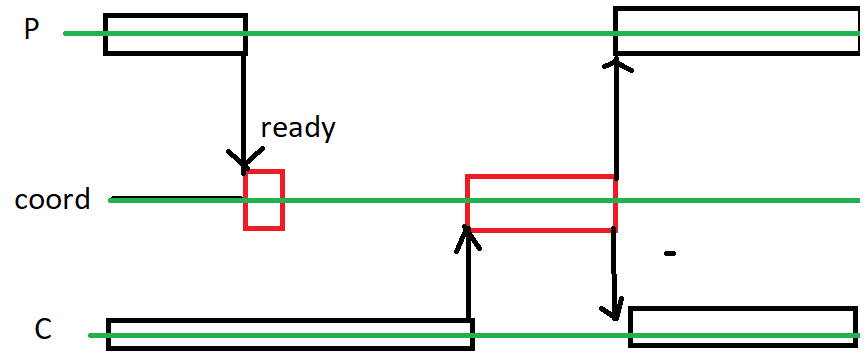
\includegraphics[width=8cm]{sequence.png}
	\caption[Thread activity with an event-handling coordinator.]{TODO. Figure is placeholder too.}
	\label{fig:sequence_diag}
\end{figure}

One pivotal decision of our final design is to attempt to alleviate this problem. If compute-threads are going to block, waiting for progress anyway, why not have them do the coordination \textit{themselves}? In our approach, we discard the dedicated protocol thread and re-interpret the coordinator as a \textit{role} which the other threads take turns adopting. Conceptually, this change is a minor one; there is ultimately still at most one thread acting as coordinator. Until now, we have taken for granted that the coordinator can complete interactions with impunity; as they are the only elected leader of their kind, there is no concern for data races. In our new model, if \textit{anyone} can be a coordinator, we must go our of our way to prevent two threads from adopting the role at once. Where before the bottleneck existed (implicitly) as a single coordinator thread processing a sequence of events \textit{one at a time}, we now make the lock explicit: upon becoming ready, every thread attempts to acquire the \textit{protocol lock}, the holder of which acts is the only coordinator for the duration.

\subsubsection{Delegating the Task of Data Exchange}
Owing to our focus on values at the systems level, we do not have the simplifying luxury of the Java backend to presume that moving data is cheap. In Rust, as in C and C++, values are not represented by indirect references by default; often, their shallowest representations are all there is to them. To satisfy $\boldsymbol{R^N_{data}}$, the Java backend's (admittedly intuitive) representation of ports as data pigeonholes is wasteful. For many realistic Reo protocols, data often moves \textit{through} protocols synchronously, moving from \code{Putter} to \code{Getter} without any storage in memory cells in-between. 

Our implementation introduces a new idea in an attempt to capitalize on this observation: getters fetch their data directly from the \textit{source}. In this approach, the coordinator does necessarily handle data itself. Rather, it decides which rule to fire and \textit{delegates} the task of moving the data to the getters themselves. In addition to skipping a redundant `data hop' from putter to coordinator, this also facilitates the dissemination of a putter's datum to all its getters \textit{in parallel}. This change requires extra messaging form the coordinator, as getters are given more responsibility. Where before a signal from coordinator to getter sufficed (`Your datum is ready!'), coordinators must now communicate the location of the getters' source (`Your datum can be found at $P$!').


\subsection{Architecture}
\label{sec:protocol_object_architecture}
\code{Proto} is a type corresponding closely to its imperative-form specification type, \code{ProtoDef}. While they represent the same thing, their differences in structure and contents are a result of them being used for different \textit{purposes}. Despite the increase in granularity from Reo's RBA-like form, \code{ProtoDef} still represents a \textit{specification} of the protocol; as such, it strives to minimize redundancy to simplify parsing and minimize the surface for internal inconsistency. On the other hand, \code{Proto} is structured to facilitate \textit{execution} at runtime.

\begin{enumerate}
	\item \textbf{Layout optimized for speed.}\\
	As discussed in Section~\ref{sec:imperative_to_rust}, the \code{build} method is the only user-accessible means of constructing \code{Proto} instances. The methods of this type can rely on this to assume that their contents are internally consistent, thereby avoiding the cost of performing many checks at runtime. For example, if a \textit{rule guard} includes an equality check between the values in memory cells $m_0$ and $m_1$, \code{Proto} is able to assume that these cells have the same type; it is safe to use the result of $m_0$'s definition of type-equality.
	
	Additionally, concise structures can be re-arranged such that their layout facilitates less computation time. A general example of this paradigm is caching. Here, a clear example is the replacement with symbolic \textit{names} for ports, functions and memory cells (represented by strings in the \code{ProtoDef} type), using \textit{integers} for keying into vectors, maps and other such structures directly.
	
	\item \textbf{Additional data for primitive concurrency.}\\
	Where \code{ProtoDef} can leave information implicit, \code{Proto} must be explicit. Interface ports require some data structures for storing concurrency primitives. For example, coordinators must send \textit{control messages} to getters, as explained in Section~\ref{sec:chosen_design} above. 
\end{enumerate}

\subsubsection{Critical Region}
Section~\ref{sec:chosen_design} explains how threads initiating actions at boundary ports of a protocol assume the role of coordinator. It is fruitful to examine the fields of \code{Proto} in accordance to which \textit{roles} access them, and how their access is safely controlled. The most coarse-grained distinction is that between fields inside and outside the protocol's lock-protected \textit{critical region}. This divide is so fundamental, that is is immediately apparent by looking at the definition of \code{Proto} itself, seen in Listing~\ref{listing:proto}. \code{ProtoCr} stores all of the fields manipulated only by the coordinator, such as the \textit{allocator}, to which the coordinator delegates the task of storing persistent values. This is explained further in Section~\ref{sec:memory_cells} to follow. Also observe the field responsible for managing which ports are \textit{claimed}. While this is not a task traditionally associated with the coordinator, it's mutually-exclusive access between threads necessitates that this structure is protected by the lock.

\subsubsection{Spaces}
Clearly, \code{ProtoCr} can contain only the data that is not contended by multiple threads. Some structure is still needed for threads to \textit{rendezvous} such that information can be exchanged and actions can be aligned in time. In the Java implementation, the class \code{Port} served two distinct purposes: (1) stored the value being exchanged by two threads, and (2) acted as the rendezvous for putter and getter. As explained in Section~\ref{sec:chosen_design} above, the former of these tasks does not involve the coordinator in Reo-rs. However, the latter is still relevant. To meet this need, \code{ProtoR} associates \textit{space} for every identifier (for ports and memory cells alike). The difference is name exists to distinguish them from ports, to which they are certainly related, but not identical. For every identifier, its \code{Space} contains precisely the data needed for it to communicate with its peers. For ports, this includes a \code{MsgBox}, which serves as a control-message channel from coordinator to compute-thread. Spaces are discussed further in Section~\ref{sec:data_exchange} to follow. 

\begin{listing}[ht]
	\centering
	\inputminted{rust}{proto.rs}
	\caption[Proto type with parts inside and outside the lock.]{Definitions of the most coarse-grained structures of a protocol instance. \code{Proto} is the entry-point, composed of \code{ProtoCr} in the critical section, accessed by only the coordinator, and \code{ProtoR} outside it, accessed by all.}
	\label{listing:proto}
\end{listing}


\subsection{Behavior}
\label{sec:behavior_implementation}
This section explains how the data structures of the \code{Proto} type comes to life at runtime to emerge as coordination according to the protocol with which it was configured. 

\subsubsection{Rule Interpreter}
Unlike the Java implementation, Reo-rs moves the specification of the protocol type very late into the pipeline from Reo to the final application. Rather than relying on Reo to generate \textit{native} application code, in this work we make more extensive use of the \textit{virtualization} pattern. At runtime, the coordinator traverses rules in data form, performing tasks as a rudimentary \textit{interpreter}. The tasks associated with such a \code{Rule} correspond closely to the conceptual interpretation of the imperative form; as such, they are treated like \textit{transactions} at runtime. 

\hl{TODO more detail and talk about temporary variables}


\subsubsection{Minimizing the Bottleneck}
\label{sec:minimizing_the_bottleneck}
Reo-rs shares its centralized locking architecture with the Java back-end. Regardless of whether the coordinator and the thread that performs the role are decoupled, the importance of providing it mutual exclusion is clear; two coordinators in tandem would not be safe in the knowledge that the state does not change between evaluating the guards and changing the state. Methods exist for \textit{fragmenting} protocols such that the locking becomes finer grained as protocols are into sets of smaller ones. As such, the Reo compiler internally produces a \textit{protocol set} as its output, though the work on this feature is ongoing. Nevertheless, we consider this decomposition an orthogonal concern and consider it no farther. Reo-rs embraces this central lock, but takes measures to minimize the duration for which it is held. In this section we discuss these measures and how they work together to help satisfy $\boldsymbol{R^N_{fast}}$. To structure our reasoning, we identify the tasks a coordinator performs from the moment to acquires the lock (accepting its role), to the moment it releases it (relinquishing the role). 

\begin{enumerate}
	\item \textbf{Initialization}\\
	Section~\ref{sec:port_operations} explains how the time spent purely on \textit{overhead} is diminished by avoiding the event-signal interaction used by the Java implementation, necessary to wake a sleeping protocol thread. Once the coordinator has acquired its lock (a task needed in both versions), transitioning into the work of the coordinator is nothing more than the time taken to invoke the \code{coordinate} function call.
	
	\item \textbf{Checking Readiness and Memory State}\\
	Imperative form shares the explicit representation of the \textit{synchronization set} with RBAs, encoding precisely which ports are involved with the firing. Clearly, a rule cannot fire until all ports involved are \textit{ready}. Per port, this is a boolean property which can be represented by a single bit flag. Owing to the simplicity of this data, each of these sets can be represented as a single \textit{bit-vector}, a data structure for which set-operations are exceptionally fast. Reo-rs takes this optimization a step further by extracting another boolean property per memory cell: \textit{fullness}. The idiomatic encoding for memory cells storing data of type \code{T} in Rust would be the \code{Option<T>} type, such that \code{Option::None} represents \textit{emptiness}. Instead, the relevant flags for fullness are extracted, separated from their data and instead coalesced into another bit-vector. With just a handful of fast bit-wise operations, the coordinator is able to quickly detect whether a rule \textit{cannot} fire, as a result of a port not being ready, or a memory cell being full when it should be empty, or empty when it should be full. In practice, the vast majority of cases where a rule's guard is unsatisfied are detected in this step.
	
	
	\item \textbf{Instructions}\\
	Instructions are relatively expensive compared to the other steps in a rule's interpretation. Their cost scales with their complexity, as they can be defined as arbitrarily large and deep formula terms. Even individually, the cost of each operation can be high, as they include arbitrary user-defined function invocations, arbitrary user-defined equality checks, and allocation space for newly-created data objects. Section~\ref{sec:memory_cells} explains how the cost of memory allocation is mitigated such that the allocation itself is amortized to constant time. For the rest of these operations, there is not much that can be done to avoid the cost; for the most part, they would be expensive even if each rule were performed by a native Rust function. Fortunately, the vast majority of rules for Reo connectors require no instructions at all. In practice, Reo connectors tend not to \textit{inspect} the data whose flow they coordinate. The more intrusive the protocol's routing logic becomes, the more it begins to resemble \textit{computation}, a task for which Reo should probably not be optimized. For the protocols without instructions (including \textit{fifo1}, \textit{alternator}, \textit{sequencers}, \textit{sync}, \textit{lossy sync} and more), the support for instruction parsing costs no more than the time to determine that there are zero instructions to execute.
	 
	 \item \textbf{Movements}\\
	 Once a rule is committed, the role of the coordinator is to kick any getters into action, delegating the data exchange to them. Each \textit{movement} encodes one \textit{resource} (\code{Putter} or memory cell) being distributed amongst a set of \textit{recipients} (each a \code{Getter} or memory cell). This meta-interaction is not synchronous; getters may take arbitrary time before waking up and actually participating in the data exchange. This is not the case for memory cells; as part of the \textit{state} of the protocol, this is manipulated by the coordinator only. As such, operations which move values \textit{into} memory (where memory cells act as getters) are performed first. Section~\ref{sec:memory_cells} explains this procedure in more detail. Here, it suffices to say that the movement of memory between memory cells is fast.
	 
	 For port-getters, the coordinator does not move the value itself. Rather, the work is delegated to the compute-thread by sending a \textit{control message} to the getter's \code{MsgBox}. 
	 
	 Usually, the coordinator does not have to interact with the resource (acting as putter) at all. It can rely on getters to `clean up'. The coordinator returns, releasing the protocol lock. The only exception is for movements with \textit{zero getters}. Such cases can represent a resource being destroyed. In these cases, there is no getter to perform the cleanup, and so, the coordinator does it itself. For a \code{Putter}, this is no more than sending a control message, releasing it. For memory cells, this may require running the \textit{destruction} function associated with the memory cell's data type.  Section~\ref{sec:memory_cells} provides more detail on how these are managed.
	 	
\end{enumerate}

\subsubsection{Data Exchange}
\label{sec:data_exchange}

Eventually, each \code{Getter} waiting at their \code{MsgBox} receives a control message from the coordinator, revealing to them the identity of their \textit{resource}. Their task is to locate the corresponding \code{Space} and contend with an unknown number of fellow getters to complete the \textit{movement}. The correctness of this exchange relies on the satisfaction of a number of properties:
\begin{enumerate}
	\item \textbf{One getter cleans up the resource}\\
	Regardless of whether the resource is a \code{Putter} or a memory cell, the set of getters are responsible for cleaning up the resource to finish the interaction. In the case of a putter, this takes the form of sending them a \textit{control message}, notifying them that everyone has finished inspecting their datum and they may return to the caller. Clearly it is unsafe for anyone to release the putter \textit{before} some getter has finished reading the datum; by returning, the putter may \textit{invalidate} the memory region storing the datum.
	
	In the case of a memory cell resource, cleanup takes the form of re-setting its \textit{ready flag} inside \code{ProtoCr}, signifying that the memory cell is in a stable state can again be involved in rule firings. This is necessary as there is no dedicated thread guaranteed to set this flag in future, as is the case for getters and putters. Section~\ref{sec:memory_cells} to follow also explains how these memory cells are \textit{emptied} in these events such that they can again store new values. This manipulates the protocol's state, potentially making new rules' guards satisfiable. As such, this last getter must once again acquire the protocol lock and attempt to \textit{coordinate}.
	
	\item \textbf{At least $N-1$ getters \code{clone}}\\
	Rust generalizes the operation for \textit{replicating} a datum to produce another instance from it. It is idiomatic to rely on the standard trait \code{Clone} with single operation \code{clone} to implement this behavior. This approach covers cases for which there is a non-trivial means of replicating objects; sometimes, performing a bit-wise copy of the structure's shallowest representation is not enough. Consider the example of \code{Arc} (`atomic reference-counted') in Rust's standard library. This type consists of just a pointer to some heap-allocated tuple \code{(refcount, data)}, and is used for shared, reference-counted ownership of \code{data}. For this type, coping the pointer to the tuple is not sufficient. Cloning must \textit{follow} the pointer and increment \code{refcount}.
	
	\item \textbf{One getter \textit{moves} instead of cloning}\\
	Data movements represent the \textit{transmission} of data from source to a set of destinations. Generally, the value is no longer present at the source afterwards. Na\"ively, the original must be \textit{destroyed} to complete the interaction. However, it is wasteful and illogical to replicate an object only to destroy the original. Instead, we wish to \textit{move} a value between threads, much as Rust's move semantics allow the movement of affine types between bindings. This cannot be done in the conventional way, as movement is defined is generally within the context of a single thread and scope. Regardless of Rust's expressiveness, it is nonetheless an \textit{action-based} language, and does not offer the \textit{interaction} we need.\footnote{Rust is able to understand uni-directional movement of values into \textit{new} threads using the same mechanism by which closures can \textit{enclose} variables in their parent scope. More complex types are able to also create their own notions of safe `movement' by composing actions as we suggest in this section. As in our case, they require the use of \code{unsafe}, as by definition the Rust compiler cannot reason about their correctness in the usual way.}
	
	When orchestrated correctly, we are able to implement a safe \textit{move} operation between threads by invoking a pair of \textit{unsafe} operations, one on either end. In \textit{unsafe Rust} it is possible to \textit{copy} a value without influencing the original. If not done correctly, this can easily lead to \textit{double-frees}. On the other hand, it is possible to leak resource memory with \code{forget}, an operation of Rust's standard library which causes the compiler to consider the value \textit{moved} without invoking \code{drop}. These pitfalls should be familiar to C programmers, as \textit{unsafe Rust} gives one the capability to interact with \textit{raw pointers} in a fashion similar to that of C. Together, these actions constitute the inter-thread move primitive we need.
	
	We elaborate our task by requiring an election between getters, such that one is designated the \textit{mover}, and the rest are \textit{cloners}. 
	
	\item \textbf{All clones must be complete before the move}\\
	 It is unsafe to \textit{move} a value before or while performing \code{clone} on the original. Essentially, every data exchange must proceed in two strict phases such that all clones occur in the first, and the move in the second.
	 Consider again the example of type \code{Arc} by examining this sequence of events that results in undefined behavior: (1) \code{Arc} $x$ represented by a pointer to heap region at $p$ is moved to binding $y$. (2) $y$ goes out of scope, it's \code{refcount} is reduced to zero, and so its heap allocation is freed. (3) \code{Arc::clone} is invoked with $x$, which traverses its pointer to memory position $p$, and attempts to increment \code{refcount}. $p$ is no longer allocated, and arbitrary memory corruption ensues. To prevent such cases, Reo-rs must take care to order all clones of some value before it can be moved, as the Rust compiler would do.
\end{enumerate}

Many solutions are possible, but have in common that these getters must exchange some meta-information safely across thread boundaries. Our solution uses a pair of atomic variables for this purpose, \textit{count} and \textit{mover}, initialized by the coordinator a priori to $N$ and \textit{true} respectively. In a nutshell, \textit{mover} is true if no getter has yet claimed the role of mover, which represents both (1) the responsibility to clean up, and (2) the privilege of moving the original value, rather than cloning it. Part of the procedure at large is a \textit{pair} of \textit{elections} between getters to determine a \textit{mover} and a \textit{last} getter. We elect a mover first. The time between the elections gives the losers (the `cloners') the opportunity to clone, safe in the knowledge that the mover will not clean up until they are finished. If the mover is also elected last, they clean up and return immediately, as all clones must already be complete. Otherwise, the mover must await a signal from whomever is last before cleaning up.

This process is complete enough to implement the desired functionality for \mbox{Reo-rs}. However, we identify two important optimization opportunities which have the unfortunate consequence of complicating the data-exchange procedure further.
\begin{enumerate}
	\item \textbf{Not all getters want data}\\
	Getters participating as a result of the \code{get\_signal} operation will not return a value. Clearly these getters cannot avoid participating in the mover-election, as then nobody would clean up. These getters specialize their interactions by participating in the last-election first. The intuition is that if they lose this election, it is safe for them to return without participating in the mover-election; clearly this covers the case of no getters wanting the data. It is also safe to re-arrange these elections in this case; these getters have no intention to \code{clone}, and thus are not a threat to the invariant that required these elections to be ordered in the first place: all clones are complete by the time the last-getter is
	
	\item \textbf{\code{Copy}-types can be replicated without \code{clone}}\\
	Section~\ref{sec:rust_language} explains how \code{Copy} marks types for which have a trivial destructor, and are safe for multiple getters to replicate by \textit{copying} their value bit-wise. This is the case for primitives, and structures composed entirely out of primitives, such as arrays of integers. 
	
	For copy-types, the mover and the \textit{copiers} may copy the original datum in parallel. Afterward, only a last-getter is elected to clean up, safe in the knowledge that all copies are finished.
\end{enumerate}

The full data-exchange procedure is spelled out in Rust-like pseudocode in Listing~\ref{sec:data_exchange} in the Appendix.

% (1) getters invoked by \code{get\_signal}  //
%
%
%Another optimization exists for cases where the data type implements the \code{Copy} trait, communicating that this type has a trivial destructor, and it is perfectly safe for multiple getters to \textit{copy} the data by replicating its shallowest representation in parallel. This is the case for primitives, and structures composed entirely out of primitives, such as arrays of integers. For these types, each getter knows a priori that every getter will conclude that the type implements \code{Copy}, and it can forgo the mover-election business. It is still necessary to elect one getter as the \textit{last} to perform the cleanup (the putter must still be released, or the memory cell must still become ready). The full procedure for a getter's role in data exchange is given in the appendix as Listing~\ref{listing:get_data}, which in and of itself demonstrates the logistic complexities that Reo-rs is able to hide from its users.



\subsubsection{Memory Cells}
\label{sec:memory_cells}
Section~\ref{sec:protocol_object_architecture} explains that per \textit{location} (generalizing ports and memory cells), Reo-rs maintains a persistent \code{Space} structure at a fixed location on the heap such that threads have a predetermined location to \textit{rendezvous} on communication primitives. Section~\ref{sec:data_exchange} follows up, explaining how these structures are also pivotal to data exchange. When getters converge on the space of a \code{Putter}, they rely on the presence of a prepared \textit{data reference} in the space to the location of the putter's datum on its own stack. In this manner, values moving between ports are never moved to the heap at all. The memory-alignment of the putters datum generally differs per data exchange, necessitating that their space's reference be \textit{updated} to the location of their value each time. 

Memory cells differ from putters in that their value \textit{persists} beyond the lifetime of any individual thread participating in the protocol; consequently, the data itself \textit{must} be stored on the heap. A na\"ive implementation treats memory cells similarly to putters by continuously \textit{updating} the data-reference in the associated \code{Space} such that it points to a freshly-allocated value on the heap every time the memory cell is filled.

We are able to rely on a property of Reo for an optimization: memory cells have pre-defined types. Instead of shifting the pointer around to a fresh allocation each time, we are able to \textit{pre-allocate} the space needed to store one value per memory cell. In this model, the references do not change. Instead, each has a single allocation which is repeatedly re-used. Whenever the cell is empty, the contents of the allocated space are \textit{uninitialized}. This can be done safely by relying on auxiliary structures for tracking when memory cells are empty; Section~\ref{sec:minimizing_the_bottleneck} explains how \textit{bit vectors} serve this purpose for Reo-rs. This approach removes the cost of creating and allocating spaces at runtime. Unfortunately, this approach suffers a drawback inherited from its strict interpretation of \textit{value-passing semantics}: moving data between memory cells is expensive. While small optimizations are possible for some circumstances (eg.\ we are able to swap references when the contents of two memory cells are \textit{swapped}), they are only applicable in a handful of situations. 

Requirements~$\boldsymbol{R^N_{data}}$ and~$\boldsymbol{R^N_{fast}}$ incentivize a more extensive optimization. Reo-rs intentionally decouples memory cells (including their spaces and their fullness flags) from \textit{storage}, which describes where the contents of the cells is kept on the heap. We observe that Reo protocols perform logical replication of values often, while mutating existing values rarely. As such, many situations exist in which we are able to safely \textit{alias} values between memory cells by relying on \textit{reference counting}. We extend the idea of re-using allocations, but rather that fixing them per memory cell, we allow all memory cells of the same data type to draw from a shared pool of re-used allocations; this is often referred to as an \textit{arena allocator}. The intricacies of this process are delegated by the coordinator to the \code{Allocator}, which tracks which \textit{storage cells} of a type are available (free) and which are occupied. Rules which replicate, destroy or move data between memory cells thus can often moving data altogether, instead manipulating only the references within spaces, and reference counters of storage cells. For example, a rule which empties memory cell $m_0$ (destroying the contents) needs to only decrement the reference counter. Only when the counter reaches zero does the allocator need to be involved, invoking the value's destructor in-place and freeing the storage slot. This approach has another advantage: \code{clone} is invoked \textit{lazily}, in some cases being avoided altogether. Consider a connector for which values originate from putters, get stored in memory slots, are replicated repeatedly, only to be destroyed before ever being emitted to a getter. In this example, \code{clone} is never necessary. This approach has an additional consequence; the data exchange operation explained in Section~\ref{sec:data_exchange} may be initialized such that \textit{nobody} is permitted to move. The procedure already given (in Listing~\ref{sec:data_exchange}) is able to handle this case.



%
%Memory cells can be \textit{empty}, in which case their pointers are \textit{dangling}\code{For safety, their pointers are managed such that they are \code{null} if and only if the memory cell is empty. This is safe, as null never represents a valid value. Reo-rs can be compiled with \textit{assertions} intact to continuously check this invariant.}. A na\"ive implementation might affix the location
%
%Reo allows the expression of \textit{stateful} protocols whose rules move data into and out of memory cells inside the protocol itself. The protocol object already stores \textit{references} to data on the stacks of port-putters, but this data is \textit{transient}, where memory cells are persistent. To play the part, each protocol object contains a \code{Storage} structure, which acts as a custom \textit{memory allocator}. As the \textit{system allocator} (familiar in C through functions \code{alloc} and \code{free}) depends on a simpler layer of system calls (\code{mmap} etc.) to provide the intended functionality, so too does the \code{Storage} rely on the system allocator. This special type has much the same functionality of the system allocator, but is designed to take advantage of a non-trivial property of Reo protocols: We at most require one allocation per memory cell, and we know the required memory size and alignment ahead of time, as these cells are typed. Thus, \code{Storage} will make a constant number of system-allocations at runtime, re-using the allocated slots as data is moved in and out.
%
%As both the behavior of the coordinator and the allocator are under the control of Reo-rs, it is safe to represent values in memory cells with a layer of indirection between a \textit{memory cell} (a variable that is involved with guards and rules), and \textit{storage cell} (A chunk of memory reserved by the allocator). Regardless of the size of the data itself, `moving' it between memory cells is an instance of \textit{reference passing}.
%
%This approach can be easily extended to facilitate a powerful optimization: \textit{aliasing}. In practice, it is common for Reo to replicate data without mutating either replica. Until the replicas diverge, it is perfectly correct to \textit{alias} the original memory cell by copying its storage-cell reference. Here, the contents of a storage cell are only moved out again if the reference to it is \textit{unique}. This necessitates \textit{reference counting}.
%
%Observe that this approach allows us to \textit{delay} the cost of the \code{clone} operation, avoiding it entirely in cases where the clone is never mutated nor moved out of protocol memory before being discarded; ie. aliased references are made independent with \code{clone} \textit{lazily}. The logical extreme of this idea is to avoid unnecessary clones entirely, covering cases where a value is cloned into memory from a putter, and then discarded. (TODO) Our solution relies on the Reo compiler's minimization procedure to remove these data-movements when the value is \textit{statically} guaranteed to be discarded before use. Supporting the \code{get\_signal} operation described in Section~\ref{sec:port_features} prevents us from avoiding these clones where their values are discarded \textit{dynamically}, as the choice of whether it will be used is not decided until \textit{after} the putter has returned, invalidating the original datum.
%\hl{
%memory cells clearly outlive the stacks of any putters. therefore, the protocol has its own independent persistent memory on the heap. However, it does not use the system allocator directly; data moves through ports very quickly and the overhead of allocating new objects is exceptionally wasteful. instead, we leverage the information made available by the reo specification: we know ahead of time which memory allocations we will need, and we know precisely in which sizes and alignments they will be. we can allocate a fixed number of STORAGE SLOTS and then re=use them. A sensible implementation would simply assign such a slot to each MEMORY CELL SPACE and swap values in and out, initializing and uninitializing the same memory region repeatedly. Clearly, as these memory variables are of irregular sizes, this necessitates a level of indirection: spaces have POINTERS to an allocated heap space. while we are at it, a minor change provides a powerful optimization: we decouple storage slots and memory cells entirely with the addition of a custom ALLOCATOR with REFERENCE COUNTING. when a memory cell moves data to others, only the POINTER moves to its storage slot, and the refcount is updated accordingly. this makes movement and replication within the protocol trivially cheap. it also means that the cost of dropping values is postponed until the last possible moment: the `original' is destroyed only when the LAST memory cell removes its reference.
%}



\subsubsection{Type Reflection}
\label{type_reflection}




Section~\ref{sec:rust_language} explains how Rust offers both \textit{static} and \textit{dynamic} dispatch for executing generic code, similar to how it is done for C++. These options offer a trade-off in runtime speed, binary size and flexibility. The interpreter approach taken by Reo-rs makes it difficult to make effective use of static dispatch, as this requires that the concrete type be known at the \textit{call site}. While it is common for Rust libraries to be written in terms of generic arguments which the user will statically dispatch in their own code, this is not particularly ergonomic in our case. As their types are distinguished by context alone, it is impossible to store generic types together in typical collections (such as maps or arrays). This presents a problem for defining objects for generic Reo protocols, which vary also \textit{number} and \textit{arrangement} of data types. 

Cases such as ours which require more extensive flexibility usually rely on dynamic dispatch instead. With this approach, generic type parameters behave less like static \textit{macros}, and more like \textit{interfaces} in Java, whose virtual functions are resolved at runtime. 
As Java interfaces define their virtual functions, Rust achieves dynamic dispatch by hiding some concrete type behind a particular \textit{trait}, which provides the interface henceforth. Appropriately, the Rust term for these dynamic objects is \textit{trait objects}, identifiable by the keyword \code{dyn}, for example, \code{Box<dyn Foo>}. In our case, we define trait \code{PortData} to encapsulate precisely the operations Reo needs: (1) a function for checking equality, (2) an accessor function for the concrete type's \textit{layout}, which allows us to create new heap allocations, (3) the type's destructor, and (4) the associated \code{clone} operation. These type-specific operations are distinguished at runtime by traversing \textit{virtual function tables} of the data types to resolve their specific functions. This lookup incurs some extra overhead at runtime, but we argue why this is acceptable for Reo-rs:
\begin{enumerate}
	\item \textbf{Only pay for what you use}\\
	The most significant argument in favor of dynamic dispatch for our case is the observation that the only significant downside, the added overhead to type-specific operations, are seldom incurred. Much of the work performed by the coordinator is agnostic to the data-type. Section~\ref{sec:data_exchange} explains how usually getters perform moves themselves, while coordinators interact with spaces, send messages and compare bit vectors. Furthermore, usually the argument in favor of reducing overhead is in the context of \textit{hot path} computation; one wouldn't use dynamic dispatch to compute force vectors between every pair of atoms in a physics simulation, as these would dominate the computation. Protocols are low level but simply not \textit{that} low.
	
	\item \textbf{Reduced binary size}\\
	In some cases virtualization is able to \textit{increase} performance indirectly by reducing the overall size and heterogeneity of the binary. When a program has enough different port types, static dispatch would (statically) cause a lot of code replication that interacts poorly with the \textit{instruction cache}.
	
	\item \textbf{Data type can change at runtime}\\
	Dynamic dispatch is a method of relegating the task of distinguishing type behavior to runtime by relying on \textit{data} to distinguish types. Regardless of whether this is done by necessity, this opens up new opportunities for \textit{changing} behavior at runtime. If you change the data, you change the behavior. Projects beyond the scope of this thesis may rely on dynamic dispatch to implement \textit{dynamic reconfiguration}. In a sense, the interpreter approach taken by Reo-rs represents this idea taken to the extreme: changing the contents of the \code{Proto} is able to influence more than just the \textit{types} of protocol rules, but alter them altogether.
\end{enumerate}

Rust's chosen representation of trait objects is the \textit{fat pointer}, which is able to represent an indirect object by appending a \textit{virtual function table} (`vtable'). These two pointers can be thought of as representing the data and behavior respectively. The necessity for the data itself being accessed via indirection is clear; objects implementing the trait may have different sizes in memory, but these sizes must be unified to create a common trait object with a known size. The second pointer is used by Rust `under the hood' to access the concrete functions of the original object such that it's data is accessed by functions of the correct concrete type. These trait objects can be thought to carry their behavior around with them by moving with their vtables. While ergonomic in general, this is often redundant in the case of Reo, where values are guaranteed to only move between ports and memory cells of the same type anyway. In our case, vtable pointers would be repeatedly overwritten by the same vtable pointer, coupled to a new datum. Instead, we split these pointers, and store the vtables at fixed positions; one per memory cell, and some in the \textit{allocator}. In this manner, we are able to use Rust's native dynamic dispatch, but move only \textit{data} around as is done with static dispatch. 

Our internal use of dynamic dispatch is not visible to the user. The API of putters and getters uses \textit{static dispatch} instead, as it is most suitable for the context; port objects retain the same type throughout their lifetimes. We rely on a custom type, \code{TypeInfo}, to bridge the gap. This type serves a dual purpose: (1) it acts as a key, which can be checked for equality, and (2) it \textit{contains} the vtable of the type it represents. Listing~\ref{listing:reflection} shows the \code{TypeInfo::of} function, which is the user's only means of creating new \code{TypeInfo} instances. This function is used by the user themselves to \textit{specify} the types of in the Rust-representation of a protocol's \textit{imperative form}, \code{ProtoDef}. It is used once more inside the \code{claim} function for creating a new \code{Putter} and \code{Getter}, which guarantees that the new port object represents a logical port associated with a matching \code{TypeInfo}.



\begin{listing}[ht]
	\centering
	\inputminted{rust}{reflection.rs}
	\caption[Tricking Rust into exposing a vtable.]{`Tricking' the Rust compiler into retrieving the vtable of a given type \code{T} for dynamic dispatch to virtual functions of trait \code{PortDatum}. The safe cast on line~7 inserts a pointer to a vtable which the compiler will ensure is present in the program text. \code{TypeInfo} structures can later be used for type reflection, by manually appending this pointer to reconstruct the \textit{fat pointers} that Rust natively uses for dynamic dispatch.}
	\label{listing:reflection}
\end{listing}

\code{TypeInfo::of} works by extracting an object's vtable from the text section of the generated binary, which Rust will guarantee is included by virtue of being used. To demonstrate how this works at runtime, we see the assembly generated for the \code{TypeInfo::of} function with an extremely simplified version of \code{PortDatum} consists of only function \code{get\_num}, where \code{u32} implements the trait with \code{fn~get\_num(\&self)~->~usize\{45\}}. Listing~\ref{listing:reflection2} shows the result of compilation where \code{main} returns the \code{TypeInfo} for~\code{u32}. Here, \code{.L\_\_unnamed\_1} shows the text region of the compiled binary containing a 24-byte-long vtable for \code{u32} when dynamically dispatched as implementors of trait \code{PortDatum}. In Rust, all vtables carry information about the type's \textit{layout} (\code{u32} occupies 4 bytes, and must be 4-byte aligned in memory), as well as a pointer to its \code{drop} function for deallocation (which for \code{u32} is trivial, simply returning). The remaining field points to the single function pointer associated with the trait, returning 45 as expected.  

\begin{listing}[ht]
	\centering
	\inputminted{text}{reflection2.rs}
	\caption[Example of assembly generated for extracting a vtable.]{The resulting assembly showing the vtable of type~\code{u32} for dynamic dispatch of trait \code{PortDatum} (here simplified to only having a single function `\code{get\_num}', returning an integer). Function \code{main} is exposed, creating and returning the \code{TypeInfo} of type~\code{u32} using the function shown in Listing~\ref{listing:reflection}. Observe how this function simply returns \code{.L\_\_unnamed\_1}, the vtable of \code{u32}, included by the Rust compiler.}
	\label{listing:reflection2}
\end{listing}

